% !TEX program = xelatex
% 本科综合设计（论文）开题报告（详细版）
% 编译：xelatex main.tex （运行两遍）
\documentclass[12pt, a4paper]{ctexart}
\usepackage[a4paper, top=2.6cm, bottom=2.6cm, left=2.8cm, right=2.8cm]{geometry}
\usepackage{amsmath, amssymb, bm}
\usepackage{graphicx}
\usepackage{booktabs, multirow}
\usepackage{caption}
\usepackage[subrefformat=parens]{subcaption}
\usepackage{float}
\usepackage{xcolor}
\usepackage{tikz}
\usetikzlibrary{arrows.meta, positioning, shapes.geometric, fit, calc}
\graphicspath{{figures/}}

\linespread{1.4}
\emergencystretch=3em
\captionsetup{font=small, labelfont=bf}
\captionsetup[sub]{font=small}

% 章节标题：一、 / （一）
\ctexset{
  section = {format = {\heiti\zihao{4}}, name = {,、}, number = \chinese{section}, aftername = {}, beforeskip = 1.0ex plus .2ex, afterskip = .6ex plus .2ex},
  subsection = {format = {\heiti\zihao{-4}}, name = {（,）}, number = \chinese{subsection}, aftername = {}, beforeskip = .8ex plus .2ex, afterskip = .4ex plus .2ex},
}

\begin{document}

%======================= 封面 =======================
\begin{titlepage}
\begin{center}
\vspace*{1.2cm}
{\zihao{2}\heiti 本科综合设计（论文）开题报告}\\[2.2cm]
{\zihao{4}
\renewcommand{\arraystretch}{2.0}
\begin{tabular}{r@{}l}
题　目 & \underline{\makebox[9.6cm][c]{\zihao{-4}\heiti 基于条件扩散模型的NGSO星座星地信道}}\\
       & \underline{\makebox[9.6cm][c]{\zihao{-4}\heiti 生成建模及与CGAN的对比研究}}\\
专　业 & \underline{\makebox[9.6cm][c]{}}\\
学　生 & \underline{\makebox[9.6cm][c]{}}\\
学　号 & \underline{\makebox[9.6cm][c]{}}\\
指导教师 & \underline{\makebox[9.6cm][c]{}}\\
日　期 & \underline{\makebox[9.6cm][c]{}}\\
\end{tabular}}\\[2.6cm]
{\zihao{4} 哈尔滨工业大学教务处制}
\end{center}
\end{titlepage}

%======================= 一 =======================
\section{课题来源及研究的目的和意义}

\subsection{课题来源}
本课题来源于哈尔滨工业大学2026届本科毕业论文《基于CGAN的NGSO星座星地信道建模方法与仿真》\cite{chen2026cgan}结论部分提出的后续研究建议：“本文主要采用CGAN进行信道生成建模，后续可在相同数据集和相同评价指标下，引入扩散模型、Transformer生成模型、物理约束神经网络等方法进行对比。”本课题承接该建议，在统一数据集与统一三层评价体系下，引入条件扩散模型并与CGAN基线进行系统对比。

\subsection{研究背景}
近年来，以Starlink、OneWeb为代表的非地球静止轨道（NGSO）星座进入大规模部署阶段，星地链路已成为6G空天地一体化网络的关键组成部分。与地面信道相比，星地信道具有传播距离远、多普勒频移大、仰角快速变化、受遮蔽与降雨影响显著等特点，其准确建模是系统设计、算法验证与性能评估的前提。

传统建模手段存在明显局限。实测统计建模成本高、场景覆盖有限，且参数拟合依赖特定测量 campaign，难以迁移；射线追踪等确定性仿真方法计算开销大，难以支撑大规模蒙特卡洛验证所需的批量样本生成。以深度生成模型为代表的数据驱动方法能够从数据中学习信道统计规律，实现低成本、高保真、条件可控的信道样本生成，已成为信道建模的重要发展方向。

在生成建模范式层面，现有工作以生成对抗网络（GAN）为主。文献\cite{chen2026cgan}将条件GAN（CGAN）引入NGSO星地信道包络生成任务，取得了良好的分布拟合精度；但GAN的对抗训练机制本质上是对“单条件内分布匹配”的隐式约束，其对本课题关注的两类问题——包络序列的\textbf{时序相关结构}与\textbf{条件之间的统计一致性}——均缺乏显式保障。去噪扩散概率模型（DDPM）作为近年兴起的生成范式，训练稳定、样本覆盖度高，其迭代去噪的生成机制与信道时序结构的匹配性尚缺乏受控实验的检验。这正是本课题的出发点。

\subsection{研究目的与理论意义}
本课题的核心研究问题是：\textbf{在一维时序包络建模任务上，迭代去噪式生成（扩散模型）相对对抗式生成（CGAN），能否在保持分布拟合精度的同时显著改善时序特性保持与条件间一致性？}

本课题的理论意义在于：现有CGAN信道生成研究\cite{chen2026cgan}存在三方面不足——其一，时序特性建模能力偏弱，对抗式单步映射难以刻画包络序列的时间相关结构；其二，GAN训练依赖WGAN-GP、TTUR、EMA等多重技巧抑制不稳定，且其损失仅逐条件约束分布匹配，对条件间统计规律的一致性缺乏保障；其三，该任务上仅有GAN单一生成范式的结果，缺乏与新兴生成范式的受控对比。本课题在统一数据集与统一三层评价体系下引入条件扩散模型，系统对比两类生成范式的分布拟合与时序保持能力，为“扩散模型是否更适合时序相关信道结构建模”这一假设提供受控条件下的量化检验。

\subsection{实际意义}
本课题的实际意义在于：其一，为NGSO星地链路提供低成本、高保真、条件可控的信道包络样本生成工具，可直接支撑NTN系统设计、算法验证与性能评估；其二，产出冻结的三层评价指标库与公平对比方法论，为后续NTN信道生成建模研究提供可复用的评测基准；其三，系统测定扩散模型采样步数与生成质量、采样耗时的折中关系，为生成模型在信道仿真中的工程部署提供选型依据。

%======================= 二 =======================
\section{国内外在该方向的研究现状及分析}

\subsection{星地信道统计建模研究现状}
陆地移动卫星（LMS）信道统计建模已有四十年积累，其主流框架是\textbf{复合衰落模型}：将快衰落与慢衰落（阴影）级联建模。

Loo于1985年提出经典Loo模型\cite{loo1985statistical}，将接收复信号建模为受对数正态阴影调制的直射分量与瑞利多径分量之和，包络条件分布为Rice分布、无条件分布需对阴影变量积分。Lutz等\cite{lutz1991land}提出两状态马尔可夫模型，以“好/坏”状态切换刻画遮蔽与非遮蔽的交替，状态驻留时间服从一阶马尔可夫链。

Corazza与Vatalaro\cite{corazza1994statistical}将阴影同时作用于直射与多径分量，并将参数化为仰角$\alpha$的函数，使模型可直接推广至NGSO场景，成为NGSO星地信道建模中应用最广的统计模型。其包络$r$的PDF为Rice分布对对数正态阴影的混合：
\begin{equation}
f_r(r)=\int_0^\infty \frac{r(1+K)}{S}\,\exp\!\Big(-K-\frac{r^2(1+K)}{S}\Big)\, I_0\!\Big(2r\sqrt{\frac{K(1+K)}{S}}\Big)\,\frac{p(S)}{S}\,\mathrm{d}S,
\label{eq:corazza-pdf}
\end{equation}
其中$I_0(\cdot)$为零阶第一类Bessel函数，直射分量与多径分量共同受阴影因子$S$调制。莱斯因子$K$与阴影参数均依赖仰角：
\begin{equation}
p(\ln S)=\mathcal{N}\big(\mu(\alpha),\, h^2\sigma^2(\alpha)\big),\qquad h=\frac{\ln 10}{20}\approx 0.1151,
\label{eq:shadow}
\end{equation}
\begin{align}
K(\alpha) &= 2.731 - 0.1074\,\alpha + 0.002774\,\alpha^2, \label{eq:K-alpha}\\
\mu(\alpha) &= -2.331 + 0.1142\,\alpha - 0.001939\,\alpha^2 + 1.094\times 10^{-5}\,\alpha^3, \label{eq:mu-alpha}\\
\sigma(\alpha) &= 4.5 - 0.05\,\alpha \quad (\text{dB}), \label{eq:sigma-alpha}
\end{align}
其中$K$为线性莱斯因子，$\mu$以奈培（ nepers）计，$\sigma$为$20\lg S$的标准差（dB）。低仰角时$K$小、$\sigma$大，衰落深且分布宽；高仰角时直射分量增强，包络分布收窄并趋于Rice分布。本课题即以该模型作为参考数据生成模型。

Fontán等\cite{fontan2001statistical}基于广泛测量提出了LMS信道三态统计模型（好/中等/坏），以多状态拟合不同遮蔽环境；Abdi等\cite{abdi2003new}给出了LMS信道一阶、二阶统计量的闭式表达。标准化方面，3GPP TR 38.811\cite{3gpp38811}定义了5G非地面网络（NTN）信道模型框架，ITU-R P.618\cite{itu618}给出了地空传播预测方法，Baeza等\cite{baeza2022overview}综述了NGSO信道模型的最新进展。

总体而言，统计模型物理意义明确、计算高效，但参数依赖测量拟合、场景泛化能力有限，难以直接支撑“按需生成任意仰角条件下包络序列”的任务——其采样过程只能复现模型自身假设的分布形式，无法从更丰富的数据中学习复杂统计规律。

\subsection{基于深度生成模型的信道建模研究现状}
自Goodfellow等\cite{goodfellow2014generative}提出生成对抗网络以来，其在无线信道建模中的应用迅速展开。GAN的优化目标为极小极大博弈：
\begin{equation}
\min_G \max_D\; \mathbb{E}_{x\sim p_{\text{data}}}[\log D(x)] + \mathbb{E}_{z\sim p_z}[\log(1-D(G(z)))],
\label{eq:gan}
\end{equation}
其中$D$为判别器、$G$为以噪声$z$为输入的生成器。条件GAN（cGAN）通过向$G$与$D$注入条件信息$c$（本任务中为仰角$\alpha$）实现条件可控生成。

针对原始GAN训练不稳定、梯度消失的问题，Arjovsky等提出Wasserstein GAN，以Wasserstein距离替代JS散度作为优化目标；Gulrajani等\cite{gulrajani2017improved}进一步提出带梯度惩罚的WGAN-GP：
\begin{equation}
\min_G \max_D\; \underbrace{\mathbb{E}_{x_g}[D(x_g)] - \mathbb{E}_{x_r}[D(x_r)]}_{\text{Wasserstein估计}} + \underbrace{\lambda\,\mathbb{E}_{\hat{x}}\big[\big(\|\nabla_{\hat{x}} D(\hat{x})\|_2 - 1\big)^2\big]}_{\text{梯度惩罚 GP}},\quad \lambda=10,
\label{eq:wgangp}
\end{equation}
其中$\hat{x}$为真实样本与生成样本的随机插值。WGAN-GP配合双时间尺度学习率（TTUR）、指数滑动平均（EMA）等技巧，成为信道生成任务的主流训练框架。

Xiao等\cite{xiao2022channelgan}提出ChannelGAN，利用Wasserstein GAN生成MIMO信道矩阵；国内方面，程芳芳\cite{cheng2022gan}研究了基于GAN的无线信道建模方法，乔艳丽\cite{qiao2023leo}实现了低轨卫星移动信道建模与仿真。陈万埼\cite{chen2026cgan}将CGAN引入NGSO星地信道包络生成任务：以仰角为条件，采用WGAN-GP、TTUR与EMA等训练技巧，在Corazza数据上取得了KS统计量全部小于0.07的分布拟合精度，仰角-包络均值Spearman相关系数达0.9980；但其时序指标明显偏弱（LCR相对RMSE达0.58$\sim$0.88），且GAN类方法固有的模式崩溃与训练不稳问题仍需多重技巧抑制。

\subsection{扩散模型研究现状}
Ho等\cite{ho2020denoising}提出去噪扩散概率模型（DDPM），将生成过程建模为两阶段：\textbf{前向过程}对数据逐步添加高斯噪声，$T$步后数据退化为标准高斯；\textbf{反向过程}训练神经网络逐步去噪，从纯噪声还原数据分布。前向过程定义为马尔可夫链
\begin{equation}
q(x_t \mid x_{t-1}) = \mathcal{N}\big(x_t;\,\sqrt{1-\beta_t}\,x_{t-1},\,\beta_t \mathbf{I}\big),\qquad t=1,\dots,T,
\label{eq:forward}
\end{equation}
其中噪声 schedule $\{\beta_t\}$ 单调递增。利用重参数化可得任意时刻的闭式采样：
\begin{equation}
q(x_t \mid x_0) = \mathcal{N}\big(x_t;\,\sqrt{\bar{\alpha}_t}\,x_0,\,(1-\bar{\alpha}_t)\mathbf{I}\big),\qquad \bar{\alpha}_t=\prod_{i=1}^{t}(1-\beta_i).
\label{eq:forward-closed}
\end{equation}
反向过程以$\varepsilon$预测网络$\varepsilon_\theta$参数化，训练目标由变分下界（ELBO）化简为简洁的加权MSE：
\begin{equation}
L_{\text{simple}}(\theta) = \mathbb{E}_{t,\,x_0,\,\boldsymbol{\epsilon}}\Big[\big\|\boldsymbol{\epsilon} - \varepsilon_\theta\big(\sqrt{\bar{\alpha}_t}\,x_0 + \sqrt{1-\bar{\alpha}_t}\,\boldsymbol{\epsilon},\; t,\; c\big)\big\|_2^2\Big],
\label{eq:ddpm-loss}
\end{equation}
其中$t\sim\mathcal{U}\{1,\dots,T\}$，$\boldsymbol{\epsilon}\sim\mathcal{N}(0,\mathbf{I})$，$c$为条件（仰角）。相比式\eqref{eq:gan}的极小极大博弈，该目标为普通回归损失，\textbf{训练无对抗博弈、天然稳定}。

祖先采样（ancestral sampling）反向一步为
\begin{equation}
x_{t-1} = \frac{1}{\sqrt{\alpha_t}}\Big(x_t - \frac{\beta_t}{\sqrt{1-\bar{\alpha}_t}}\,\varepsilon_\theta(x_t, t, c)\Big) + \sqrt{\beta_t}\, z,\qquad z\sim\mathcal{N}(0,\mathbf{I}),
\label{eq:reverse}
\end{equation}
但其需要$T$步（通常$T=1000$）迭代，采样成本高。Song等\cite{song2021denoising}提出去噪扩散隐式模型（DDIM），将反向过程重新参数化为非马尔可夫形式：
\begin{equation}
\hat{x}_0 = \frac{x_t - \sqrt{1-\bar{\alpha}_t}\,\varepsilon_\theta(x_t,t,c)}{\sqrt{\bar{\alpha}_t}},\qquad
x_{t-\Delta} = \sqrt{\bar{\alpha}_{t-\Delta}}\,\hat{x}_0 + \sqrt{1-\bar{\alpha}_{t-\Delta}}\,\varepsilon_\theta(x_t,t,c),
\label{eq:ddim}
\end{equation}
当$\eta=0$时采样完全确定，且可在\textbf{同一套训练权重}上以任意步数（如20步）跳步采样，为“采样步数—生成质量—采样耗时”的折中分析提供了便利工具。Dhariwal与Nichol\cite{dhariwal2021diffusion}证明扩散模型在图像生成质量上可超越GAN，并将优势归因于其更好的分布覆盖能力与训练稳定性。

近两年，扩散模型开始进入卫星与空天信道领域：Tian与Cai\cite{tian2026scalable}结合数字高程模型与射线追踪，利用扩散模型实现环境感知的空对地信道损耗预测；Huang等\cite{huang2026physics}将物理信息数字孪生用于NTN信道估计与业务预测；Xia等\cite{xia2025leo}将潜空间扩散模型与物理信息神经网络结合用于LEO信道建模。

\subsection{研究现状分析与本课题切入点}
分析上述工作可见：文献\cite{tian2026scalable}面向信道性能预测而非包络统计生成，文献\cite{huang2026physics}解决的是信道估计问题，文献\cite{xia2025leo}未基于Corazza数据、未做仰角条件包络生成、亦未与GAN公平对比。在“仰角条件Corazza包络序列统计生成”这一具体任务上，以统一数据集和统一三层评价体系对CGAN与条件扩散模型进行公平对比的工作尚属空白。

从生成机理看，两类范式存在结构性差异：GAN通过对抗训练隐式逼近数据分布，单步前向生成效率高，但分布覆盖与训练稳定性依赖多重技巧，且损失函数不显式约束时序相关结构与条件间一致性；扩散模型通过迭代去噪显式建模数据分布的逐级细化，训练为普通回归、天然稳定，其“由粗到细”的生成机制与信道包络“慢阴影+快衰落”的多尺度时序结构存在天然的适应性，但多步迭代带来采样开销。上述差异究竟在信道建模任务上如何体现，正是本课题要通过受控实验回答的问题。

%======================= 三 =======================
\section{主要研究内容}

\subsection{Corazza参考模型数据生成管线构建}
基于Corazza-Vatalaro统计模型\cite{corazza1994statistical}构建仰角条件（20°$\sim$80°）下的包络序列参考数据生成管线。包络按式\eqref{eq:corazza-pdf}--\eqref{eq:sigma-alpha}的参数化采样，时序结构由Jakes色噪声（快衰落）与一阶IIR低通阴影（慢衰落）级联产生（详见4.2节）。对包络实施log域标准化、对仰角实施线性归一化以改善模型训练的数值条件：
\begin{equation}
x = \frac{\ln(r+\epsilon) - \mu_{\ln}}{\sigma_{\ln}},\qquad \alpha_{\text{norm}} = \frac{\alpha - 50}{30},
\label{eq:standardize}
\end{equation}
其中$\mu_{\ln},\sigma_{\ln}$由全训练集一次性估计并冻结。生成规模为$10000\times 1000$的训练数据集并予以冻结，保证后续全部实验的数据口径唯一。数据质检采用理论CDF锚定、分箱统计校验与时序特性检验相结合的方式，确保参考数据自身的统计正确性。

\subsection{三层评价指标体系构建}
构建覆盖三个层次的生成信道质量评价体系：
\textbf{L1静态分布层面}考察PDF的$L_1$距离、CDF的KS统计量、Wasserstein距离及各阶矩相对误差；
\textbf{L2时序特性层面}考察包络自相关函数（ACF）、电平穿越率（LCR）与平均衰落持续时间（AFD）；
\textbf{L3系统性能层面}考察QPSK调制下误比特率（BER）曲线的$\log_{10}$域RMSE。
另设KL/JS散度与仰角-均值Spearman相关作为跨条件泛化指标。指标定义与验收线详见4.4节。指标库配套阴性/阳性对照回归测试以验证指标自身的判别有效性，接口冻结后作为全部模型评估的统一出口，保证模型间比较的口径一致。

\subsection{CGAN基线忠实复现}
依据文献\cite{chen2026cgan}公开的网络结构与训练超参数忠实复现CGAN基线：生成器采用“时序噪声滤波”卷积结构（噪声经多层Conv1d滤波为时序包络），判别器采用大感受野卷积结构（感受野435点），训练框架为WGAN-GP+TTUR+EMA（超参数详见4.3节表2）。在7个测试仰角（20°$\sim$80°，步长10°）上逐点验收，验收线为KS统计量小于0.07、仰角-均值Spearman相关系数大于0.99。复现除验证基线可用性外，还承担一项诊断任务：\textbf{考察对抗式训练在条件区间边界与相邻条件间的一致性表现}，为两类范式的机理对比提供第一手证据。

\subsection{条件扩散模型设计与实现}
设计并实现面向一维包络序列的仰角条件去噪扩散概率模型：前向过程按式\eqref{eq:forward}--\eqref{eq:forward-closed}逐步添加高斯噪声（$T=1000$，linear schedule）；反向过程以一维U-Net作为噪声预测网络，仰角条件经特征级线性调制（FiLM）注入各残差块：
\begin{equation}
h' = (1+\gamma(\alpha)) \odot h + \beta(\alpha),
\label{eq:film}
\end{equation}
其中$\gamma(\alpha),\beta(\alpha)$为条件嵌入网络输出的逐通道仿射系数，实现条件可控生成；采样阶段引入DDIM确定性采样（式\eqref{eq:ddim}）以压缩采样步数，并定量刻画“采样步数—生成质量—采样耗时”三者间的折中关系。

\subsection{系统性对比与稳健性检验}
主对比实验在两模型共用的同一冻结训练集（Corazza参考数据）与统一指标体系下开展，从分布拟合精度、时序特性保持能力、系统性能（BER）后果、连续仰角条件泛化、训练稳定性及采样效率（吞吐、延迟与参数量）等维度进行系统性对比，归纳两类生成范式各自的能力边界与适用场景。在此基础上开展跨数据源的稳健性检验：基于物理机理的信道仿真方法生成含多维条件（仰角/频率/环境/LoS状态）的扩充数据集，并视数据获取条件引入实测信道数据，两模型分别在同一新数据集上重训并重复上述对比，以检验主要结论对训练数据分布与条件维度的稳健性。

%======================= 四 =======================
\section{研究方案与技术路线}

\subsection{总体技术路线}
本课题采用“双管线、一体系”的总体技术路线：数据管线与模型管线并行构建，统一三层评价体系贯穿全部实验环节，如图\ref{fig:route}所示。

\begin{figure}[H]
\centering
\resizebox{0.98\textwidth}{!}{%
\begin{tikzpicture}[
  font=\small, node distance=4mm and 7mm,
  box/.style={draw, rounded corners=2pt, minimum height=8mm, inner sep=4pt, align=center, fill=blue!6},
  boxg/.style={box, fill=green!8},
  boxr/.style={box, fill=red!8},
  metr/.style={draw, rounded corners=2pt, minimum height=9mm, inner sep=4pt, align=center, fill=orange!14},
  arr/.style={-{Stealth[length=2mm]}, thick},
  lab/.style={font=\small\bfseries, anchor=east}]
\node[lab] at (-4.35, 0.9) {数据管线：};
\node[box] (cor) at (-3.6, 0) {Corazza 模型\\（式\,\ref{eq:corazza-pdf}--\ref{eq:sigma-alpha}）};
\node[box, right=of cor] (gen) {时序采样\\Jakes+IIR阴影};
\node[box, right=of gen] (std) {log标准化\\式\,(\ref{eq:standardize})};
\node[boxg, right=of std] (frozen) {冻结训练集\\$10000\times1000$};
\node[boxg, below=5.5mm of frozen] (qc) {数据质检\\理论CDF锚定};
\draw[arr] (cor) -- (gen); \draw[arr] (gen) -- (std); \draw[arr] (std) -- (frozen);
\draw[arr] (frozen) -- (qc);
\node[lab] at (-4.35, -2.1) {模型管线：};
\node[boxr] (cgan) at (-2.4, -3.0) {CGAN 基线（文献\,\cite{chen2026cgan}复现）\\WGAN-GP+TTUR+EMA};
\node[boxr, right=6mm of cgan] (diff) {条件扩散模型\\1D U-Net + FiLM（式\,\ref{eq:film}）};
\draw[arr] (frozen.south) to[out=270, in=90] (diff.north);
\draw[arr] (frozen.south) to[out=250, in=60] (cgan.north east);
\node[metr, minimum width=10.8cm] (eval) at (1.35, -5.2) {统一三层评价体系：L1 静态分布\quad L2 时序特性\quad L3 系统性能\quad + 泛化/工程指标};
\draw[arr] (cgan.south) to[out=270, in=170] (eval.west);
\draw[arr] (diff.south) to[out=270, in=10] (eval.east);
\node[boxg, below=5mm of eval, minimum width=10.8cm] (out) {系统性对比结论 + 跨数据源稳健性检验 + 工程选型依据（步数—质量—耗时折中）};
\draw[arr] (eval) -- (out);
\end{tikzpicture}}
\caption{总体技术路线：双管线、一体系}
\label{fig:route}
\end{figure}

\subsection{数据管线方案}
以Corazza统计模型为参考数据源，以仰角$\alpha\in[20°,80°]$为条件生成包络序列，序列长度1000、采样率$f_s=1000$~Hz（序列时长1~s）。\textbf{时序生成机制}如图\ref{fig:corazza-mech}所示：
\begin{figure}[H]
\centering
\resizebox{\textwidth}{!}{%
\begin{tikzpicture}[font=\small, node distance=5mm and 8mm,
  box/.style={draw, rounded corners=2pt, minimum height=8mm, inner sep=4pt, align=center},
  arr/.style={-{Stealth[length=2mm]}, thick}]
\node[box] (w1) {高斯白噪声 $w_1,w_2$};
\node[box, right=of w1] (jakes) {FFT $\to$ Jakes 谱 $S(f)\propto 1/\sqrt{1-(f/f_d)^2}$ $\to$ IFFT};
\node[box, right=of jakes] (rice) {Rice 包络 $R[n]=\sqrt{(m+s_R x_1[n])^2+(s_R x_2[n])^2}$\\ $m=\sqrt{K/(K{+}1)},\ s_R=1/\sqrt{2(K{+}1)}$};
\node[box, below=6mm of jakes] (iir) {一阶 IIR 低通\\ $g[n]=(1-a)w[n]+a\,g[n-1]$};
\node[box, right=of iir] (logn) {Lognormal 阴影\\ $S[n]=\exp\!\big(\mu(\alpha)+h\sigma(\alpha) g[n]\big)$};
\node[box, fill=green!10, right=8mm of rice] (out) {复合包络\\ $r[n]=R[n]\,S[n]$};
\draw[arr] (w1) -- (jakes); \draw[arr] (jakes) -- (rice);
\draw[arr] (w1.south) to[out=270, in=180] (iir.west); \draw[arr] (iir) -- (logn);
\draw[arr] (rice) -- (out); \draw[arr] (logn.east) to[out=0, in=300] (out.south west);
\node[align=center, font=\footnotesize, anchor=north] at (jakes.south west) {快衰落：ACF $=J_0(2\pi f_d \tau)$，$f_d=50$~Hz};
\node[align=center, font=\footnotesize] at (iir.south) {$a=\exp(-1/(f_s\tau_c))$，$\tau_c=0.3$~s（慢阴影相关时间）};
\end{tikzpicture}}
\caption{Corazza 参考信道时序生成机理：快衰落（Jakes）与慢阴影（IIR低通Lognormal）级联}
\label{fig:corazza-mech}
\end{figure}

其中快衰落支路产生时间相关的Rice包络，其自相关函数为$J_0(2\pi f_d \tau)$（$f_d=50$~Hz为最大多普勒频移）；慢阴影支路经一阶IIR低通产生相关Lognormal序列，相关时间$\tau_c=0.3$~s。两支路相乘得到具有真实多尺度时序结构的复合包络。模型参数$K(\alpha),\mu(\alpha),\sigma(\alpha)$随仰角的变化如图\ref{fig:corazza-params}所示：低仰角时$K$小（直射弱）、$\mu$低、$\sigma$大（阴影强），衰落更深。

对包络实施式\eqref{eq:standardize}的log域标准化与仰角归一化，形成两模型共用的标准化模型输入。冻结数据集规格见表\ref{tab:dataset}。跨数据源稳健性检验所需的扩充数据集由同一物理机理仿真方法生成，质检标准与主数据集一致。

\begin{figure}[H]
\centering
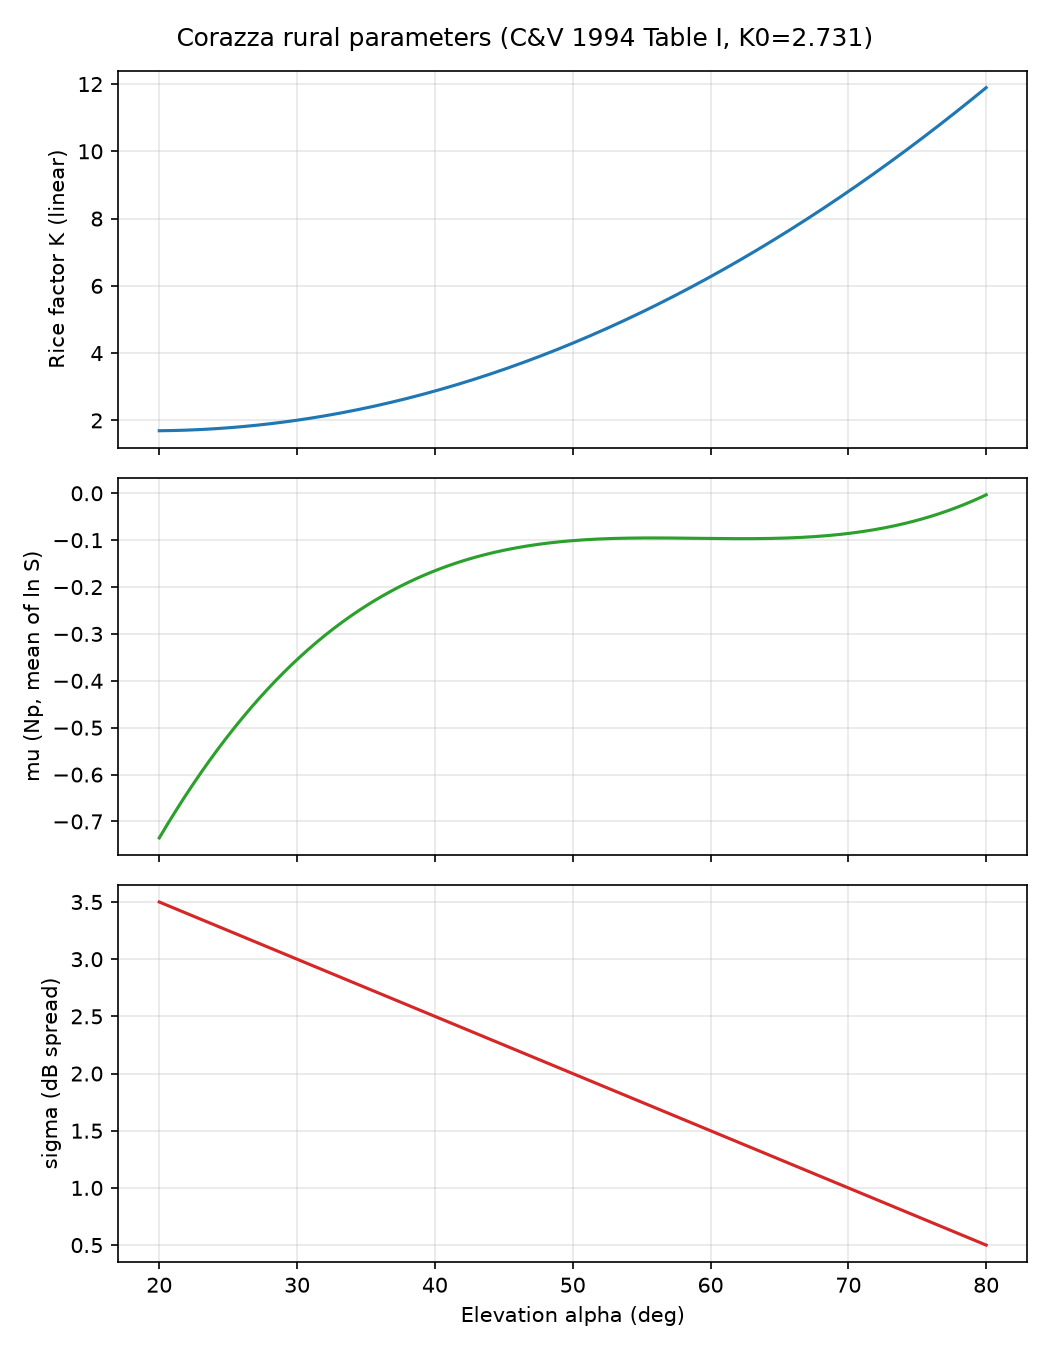
\includegraphics[width=0.72\textwidth]{corazza_params.png}
\caption{Corazza 模型参数随仰角的变化（式\,\ref{eq:K-alpha}--\ref{eq:sigma-alpha}）}
\label{fig:corazza-params}
\end{figure}

\begin{table}[H]
\centering\small
\caption{冻结训练数据集规格}
\label{tab:dataset}
\begin{tabular}{llll}
\toprule
项目 & 取值 & 项目 & 取值\\
\midrule
规模 & $10000\times 1000$（条$\times$点） & 仰角采样 & $[20°,80°]$ 连续均匀 \\
序列时长 & 1~s（$f_s=1000$~Hz） & 最大多普勒频移 & $f_d=50$~Hz \\
阴影相关时间 & $\tau_c=0.3$~s & 随机种子 & 42 \\
标准化常数 $\mu_{\ln}$ & $-0.3033$ & $\sigma_{\ln}$ & $0.5086$（$\epsilon=10^{-6}$）\\
存储精度 & float32（38.3~MB） & 用途 & 两模型共用训练集 \\
\bottomrule
\end{tabular}
\end{table}

\subsection{模型管线方案}
并行构建两个仰角条件生成模型。

\textbf{（1）CGAN对照基线。}结构如图\ref{fig:cgan-arch}所示。生成器将高斯噪声$z\in\mathbb{R}^{32\times 1000}$与仰角条件常数通道拼接后，经4层Conv1d（kernel$=15$，通道$64\to128\to128\to64$）逐层滤波，把逐时刻白噪声“滤波”为具有时间相关性的包络序列；判别器采用5层stride$=2$的Conv1d（kernel$=15$），感受野达435点（覆盖信道自相关主瓣），末端全局平均池化后输出critic分数。训练以WGAN-GP框架（式\eqref{eq:wgangp}）进行。

\begin{figure}[H]
\centering
\resizebox{0.92\textwidth}{!}{%
\begin{tikzpicture}[font=\small, node distance=4mm and 6mm,
  box/.style={draw, rounded corners=2pt, minimum height=8mm, inner sep=4pt, align=center},
  boxr/.style={box, fill=red!8},
  boxb/.style={box, fill=blue!8},
  arr/.style={-{Stealth[length=2mm]}, thick}]
\node[box] (z) {噪声 $z\sim\mathcal{N}(0,\mathbf{I})$\\ $(32\times1000)$};
\node[boxb, right=of z] (g) {生成器 $G$\\ 4$\times$Conv1d, $k$=15\\ $64\to128\to128\to64$};
\node[box, right=of g] (fake) {生成包络 $\hat{x}$\\ $(1\times1000)$};
\node[box, below=7mm of g] (cond) {仰角条件 $\alpha$（常数通道拼接）};
\node[boxr, right=10mm of fake] (d) {判别器 $D$\\ 5$\times$Conv1d, stride=2, $k$=15\\ 感受野435点 $\to$ GAP $\to$ 分数};
\node[box, right=of d] (loss) {WGAN-GP 损失\\ 式\,(\ref{eq:wgangp}) + EMA};
\draw[arr] (z) -- (g); \draw[arr] (g) -- (fake); \draw[arr] (fake) -- (d);
\draw[arr] (cond.east) to[out=0, in=200] (d.south west);
\draw[arr] (cond.west) to[out=180, in=270] (g.south west);
\draw[arr] (d) -- (loss);
\draw[arr, dashed] (loss.north) to[out=90, in=20] (g.north east);
\end{tikzpicture}}
\caption{CGAN 基线结构：时序噪声滤波生成器 + 大感受野判别器}
\label{fig:cgan-arch}
\end{figure}

\textbf{（2）条件扩散模型。}结构如图\ref{fig:diff-arch}所示。前向过程按式\eqref{eq:forward}--\eqref{eq:forward-closed}加噪（$T=1000$，linear schedule：$\beta: 10^{-4}\to 0.02$）；反向过程以一维U-Net（3级下采样$1000\to500\to250\to125$，通道$64\to128\to256$，跳跃连接，kernel$=15$与CGAN同款大核以捕捉信道自相关）为去噪网络；时间步经正弦编码+MLP逐残差块相加注入，仰角条件经FiLM（式\eqref{eq:film}）逐残差块仿射调制。训练目标为式\eqref{eq:ddpm-loss}的$\varepsilon$预测MSE；采样支持DDPM祖先采样（式\eqref{eq:reverse}）与DDIM确定性跳步（式\eqref{eq:ddim}，$\eta=0$）。

两模型的训练配置对照见表\ref{tab:hyper}。核心差异有三：目标函数（对抗博弈 vs 回归）、条件注入方式（单次通道拼接 vs 逐残差块FiLM）、采样方式（单步前向 vs 多步迭代去噪）——这三点正是后续对比实验的机理变量。

\begin{figure}[H]
\centering
\resizebox{\textwidth}{!}{%
\begin{tikzpicture}[font=\small, node distance=3.5mm and 6mm,
  box/.style={draw, rounded corners=2pt, minimum height=7.5mm, inner sep=3.5pt, align=center},
  boxb/.style={box, fill=blue!8},
  arr/.style={-{Stealth[length=2mm]}, thick}]
\node[box] (x0) {训练数据 $x_0$};
\node[box, right=5mm of x0] (fw) {前向加噪\\ 式\,(\ref{eq:forward-closed})};
\node[boxb, right=5mm of fw, minimum width=44mm] (unet) {1D U-Net $\varepsilon_\theta(x_t, t, \alpha)$\\ 3级下采样+跳跃连接，$k$=15};
\node[box, right=5mm of unet] (loss) {损失 式\,(\ref{eq:ddpm-loss})};
\node[box, below=6mm of fw] (alpha) {条件注入};
\node[boxb, below=2mm of unet] (film) {时间步 $t$：正弦编码+MLP（相加）\\ 仰角 $\alpha$：FiLM 仿射 式\,(\ref{eq:film})};
\node[box, below=8mm of film, minimum width=60mm, fill=green!10] (sample) {采样：DDPM 祖先采样 式\,(\ref{eq:reverse})（$T$=1000步）\quad / \quad DDIM 确定性跳步 式\,(\ref{eq:ddim})（20$\sim$100步，$\eta$=0）};
\draw[arr] (x0) -- (fw); \draw[arr] (fw) -- (unet); \draw[arr] (unet) -- (loss);
\draw[arr] (alpha.east) to[out=0, in=180] (film.west);
\draw[arr] (film) -- (unet);
\draw[arr] (loss.south) to[out=270, in=10] (sample.east);
\end{tikzpicture}}
\caption{条件扩散模型结构与训练/采样流程}
\label{fig:diff-arch}
\end{figure}

\begin{table}[H]
\centering\footnotesize
\caption{CGAN 与条件扩散模型训练配置对照}
\label{tab:hyper}
\resizebox{\textwidth}{!}{%
\begin{tabular}{lll}
\toprule
配置项 & CGAN基线 & 条件扩散模型\\
\midrule
目标函数 & WGAN-GP对抗损失（$\lambda_{\text{GP}}=10$） & $\varepsilon$预测MSE（式\,\ref{eq:ddpm-loss}）\\
生成网络 & 生成器4层Conv1d（$k$=15） & 1D U-Net 3级（$64\!-\!128\!-\!256$，$k$=15）\\
判别/去噪网络 & 判别器5层Conv1d stride=2（感受野435） & 同左（单一网络，无对抗）\\
条件注入 & 常数通道拼接（单次、全局） & FiLM逐残差块仿射（式\,\ref{eq:film}）\\
优化器 & Adam $\beta=(0,\,0.9)$ & Adam $\beta=(0.9,\,0.999)$\\
学习率 & TTUR：$G$ $10^{-4}$ / $D$ $3\times10^{-4}$ & $2\times10^{-4}$\\
批大小 / 训练步数 & 64 / 30000 & 64 / 30000\\
EMA衰减 & 0.999（采样一律用EMA权重） & 0.999（同左）\\
稳定技巧 & WGAN-GP+TTUR+EMA（+单调正则） & 无对抗博弈；采样时 $\hat{x}_0$ 裁剪门限30\\
采样方式 & 单次前向 & DDPM 1000步 / DDIM 20$\sim$100步\\
\bottomrule
\end{tabular}}
\end{table}

\subsection{评价体系方案}
采用统一的三层指标库，辅以连续仰角泛化指标与工程维度指标，形成“统计保真—时序结构—系统后果—工程成本”四个层面的完整评价视角。核心指标定义如下。

\textbf{L1静态分布：}设生成样本经验CDF为$\hat{F}_g$、参考CDF为$F_r$，则KS统计量、Wasserstein-1距离与PDF的$L_1$距离分别为
\begin{align}
D_{\text{KS}} &= \sup_x \big|\hat{F}_g(x) - F_r(x)\big|,\qquad
W_1 = \int_0^1 \big|\hat{F}_g^{-1}(u) - F_r^{-1}(u)\big|\,\mathrm{d}u,\notag\\
D_{L_1} &= \int \big|\hat{p}_g(x) - p_r(x)\big|\,\mathrm{d}x.
\label{eq:l1}
\end{align}
另考察均值/标准差/偏度/峰度的相对误差。

\textbf{L2时序特性：}包络自相关函数按FFT快速算法估计，取前50个滞后点的RMSE；电平穿越率（LCR）与平均衰落持续时间（AFD）在多门限$\{\gamma_\rho\}$（相对RMS电平$-20\sim0$~dB）下统计：
\begin{equation}
N_R(\gamma) = \frac{\#\{n:\, r[n]\ge\gamma,\ r[n{+}1]<\gamma\}}{T_{\text{obs}}},\qquad
T_D(\gamma) = \frac{\sum_n \mathbb{I}[r[n]<\gamma]}{f_s \cdot \#\text{穿越次数}},
\end{equation}
指标取多门限下相对RMSE。LCR/AFD属稀有事件计数统计，其相对统计误差随样本量按$1/\sqrt{N}$标度，需大样本支撑（见八(3)）。

\textbf{L3系统性能：}对生成包络序列按QPSK调制、加性高斯白噪声假设计算BER曲线（$E_b/N_0\in[0,34]$~dB），以$\log_{10}$域RMSE度量：
\begin{equation}
E_{\text{BER}} = \sqrt{\frac{1}{M}\sum_{m=1}^{M}\big(\log_{10}\text{BER}_g(\text{SNR}_m) - \log_{10}\text{BER}_r(\text{SNR}_m)\big)^2}.
\label{eq:ber}
\end{equation}

\textbf{泛化与工程指标：}KL散度$D_{\text{KL}}(p_r\|p_g)$、JS散度度量分布泛化；Spearman秩相关$\rho_s$（仰角-包络均值单调性）度量条件泛化；训练稳定性（损失曲线形态）、收敛轮数、参数量、采样吞吐与延迟构成工程维度。

指标库验收线见表\ref{tab:accept}（合格线为验收要求，优秀线为目标水平）。指标库配套\textbf{阴性/阳性对照回归测试}：以刻意劣化的伪样本验证指标能灵敏反映缺陷（阳性），以参考数据自比对验证指标不误报（阴性），接口冻结后任何变更须重跑全量回归测试并登记。

\begin{table}[H]
\centering\small
\caption{三层评价指标与验收线}
\label{tab:accept}
\begin{tabular}{llll}
\toprule
层级 & 指标 & 合格线 & 优秀线\\
\midrule
L1静态分布 & KS统计量 & $<0.07$ & $<0.02$\\
 & PDF $L_1$距离 & $<0.15$ & $<0.05$\\
 & Wasserstein距离 & $<0.05$ & $<0.015$\\
 & 矩相对误差（均值/标准差） & $<0.08$ & $<0.01$\\
L2时序特性 & ACF RMSE（前50滞后） & $<0.10$ & $<0.02$\\
 & LCR 相对RMSE & $<0.35$ & $<0.10$\\
 & AFD 相对RMSE & $<1.0$ & $<0.15$\\
L3系统性能 & BER曲线$\log_{10}$域RMSE & $<0.15$ & $<0.03$\\
泛化 & Spearman $\rho_s$ & $>0.99$ & $>0.999$\\
 & KL / JS散度 & $<0.02$ / $<0.005$ & $<0.001$ / $<10^{-4}$\\
工程 & 吞吐/延迟/参数量/训练稳定性 & 记录对比 & 记录对比\\
\bottomrule
\end{tabular}
\end{table}

\subsection{公平性保障与实验流程}
公平性保障措施（控制变量设计）：两模型使用同一冻结训练集、同一评价代码与统一的随机种子管理约定（numpy/torch/CUDA全种子固定+cuDNN确定性模式）；所有指标接口一经冻结，任何变更须重跑全量回归测试并登记，确保对比结论仅反映模型本身差异而非实验口径差异。

实验实施流程分为八个阶段：①训练集生成与冻结；②指标库自检；③CGAN训练与逐仰角验收；④条件扩散模型训练；⑤7个测试仰角逐点评测；⑥连续仰角泛化测试；⑦跨数据源稳健性检验；⑧对比分析与结论提炼。其中阶段①$\sim$③已于前期工作中完成，正式研究自阶段④开始。

%======================= 五 =======================
\section{前期工作基础与初步仿真结果}

\subsection{已完成工作概述}
开题前，本课题已按总体技术路线完成四阶段前期工作：
\textbf{阶段一}，Corazza参考模型数据生成管线：实现式\eqref{eq:corazza-pdf}--\eqref{eq:sigma-alpha}参数化与时序生成机制（图\ref{fig:corazza-mech}），完成$10000\times1000$冻结数据集与全套质检；
\textbf{阶段二}，三层评价指标库：实现表\ref{tab:accept}全部指标并通过阴性/阳性对照回归测试；
\textbf{阶段三}，CGAN基线复现：按文献\cite{chen2026cgan}超参数（表\ref{tab:hyper}）完成训练与7仰角逐点验收；
\textbf{阶段四}，条件扩散模型初步实现：完成训练与DDIM/DDPM多配置采样评估。
以下汇报各阶段关键结果与初步分析。

\subsection{参考数据管线质检结果}
图\ref{fig:corazza-pdf-cdf}给出不同仰角下生成样本的包络PDF与CDF和理论值（式\eqref{eq:corazza-pdf}数值积分）的对比：两者在高仰角与低仰角均高度吻合，验证了采样实现的统计正确性。图\ref{fig:dataset-samples}展示数据集中不同仰角的包络时序片段：低仰角（20°）衰落深、起伏大，高仰角（80°）包络稳定且集中，符合Corazza模型的物理规律（式\eqref{eq:K-alpha}--\eqref{eq:sigma-alpha}）。

\begin{figure}[H]
\centering
\begin{subfigure}{0.49\textwidth}\centering
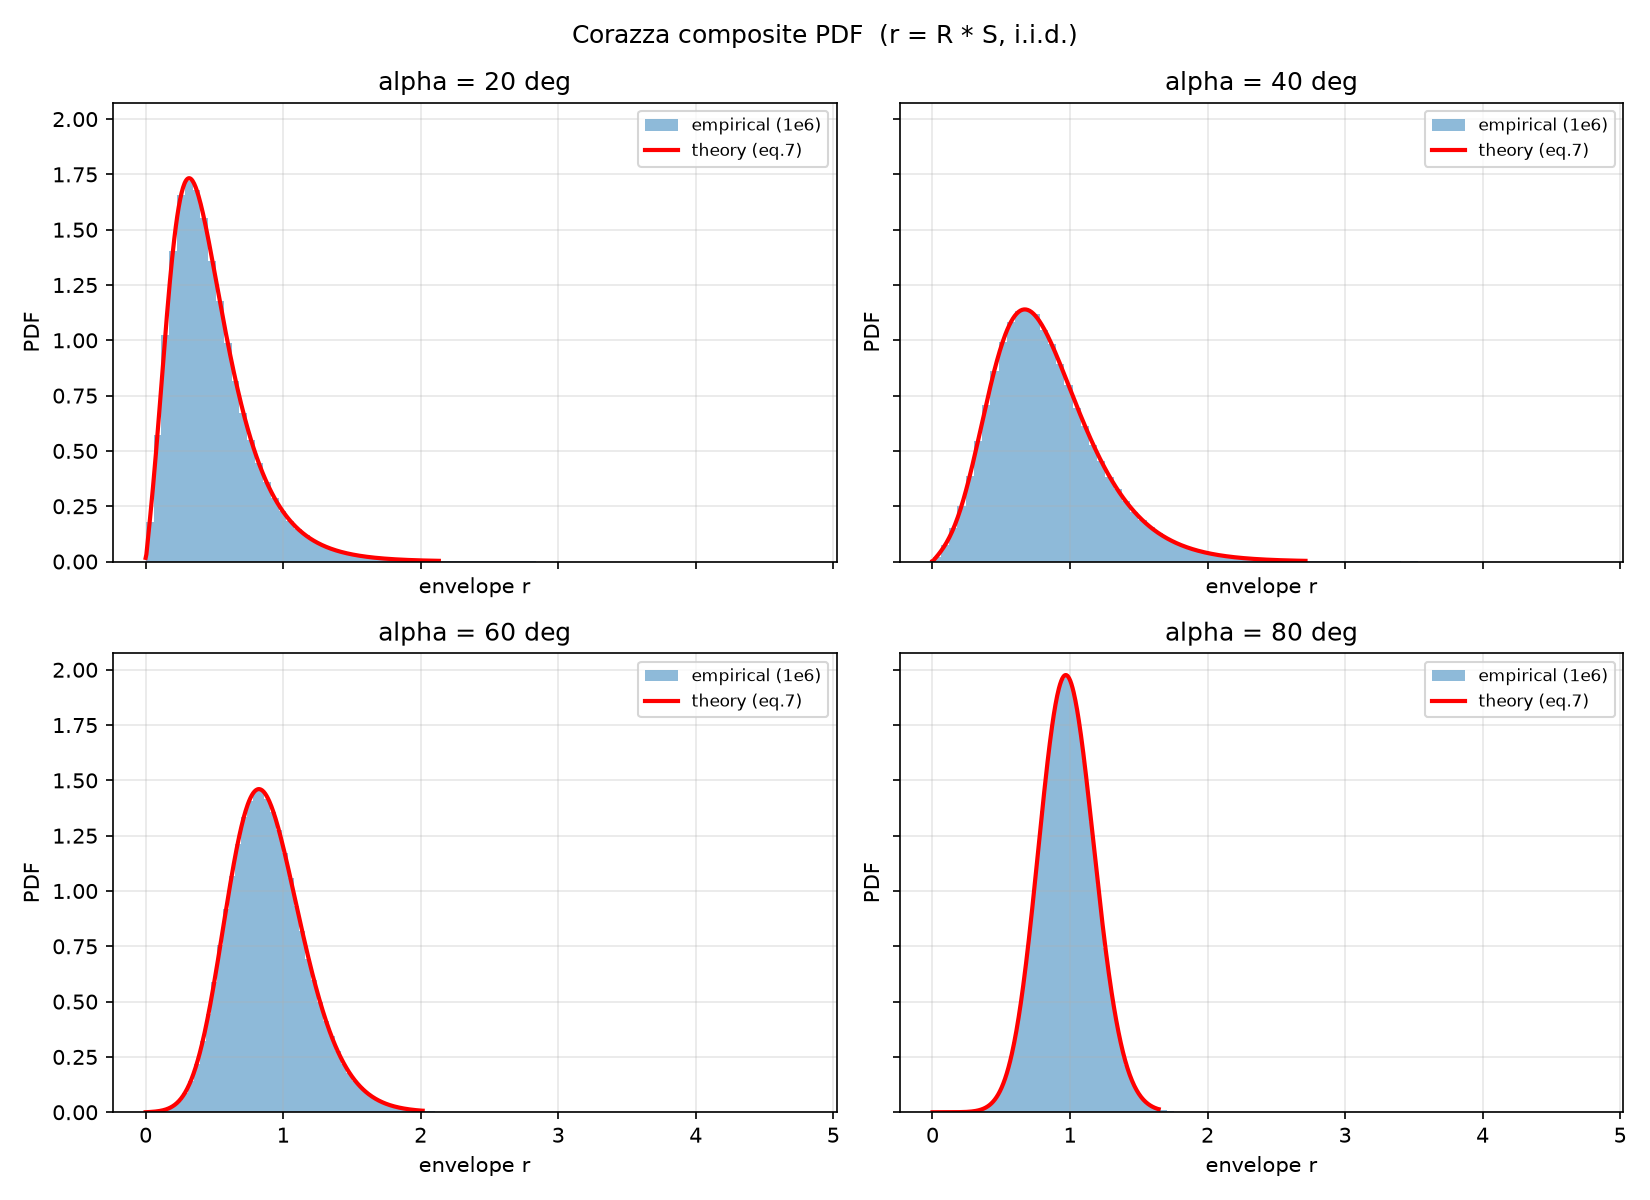
\includegraphics[width=\textwidth]{corazza_pdf.png}\caption{PDF：直方图 vs 理论曲线}\end{subfigure}
\hfill
\begin{subfigure}{0.49\textwidth}\centering
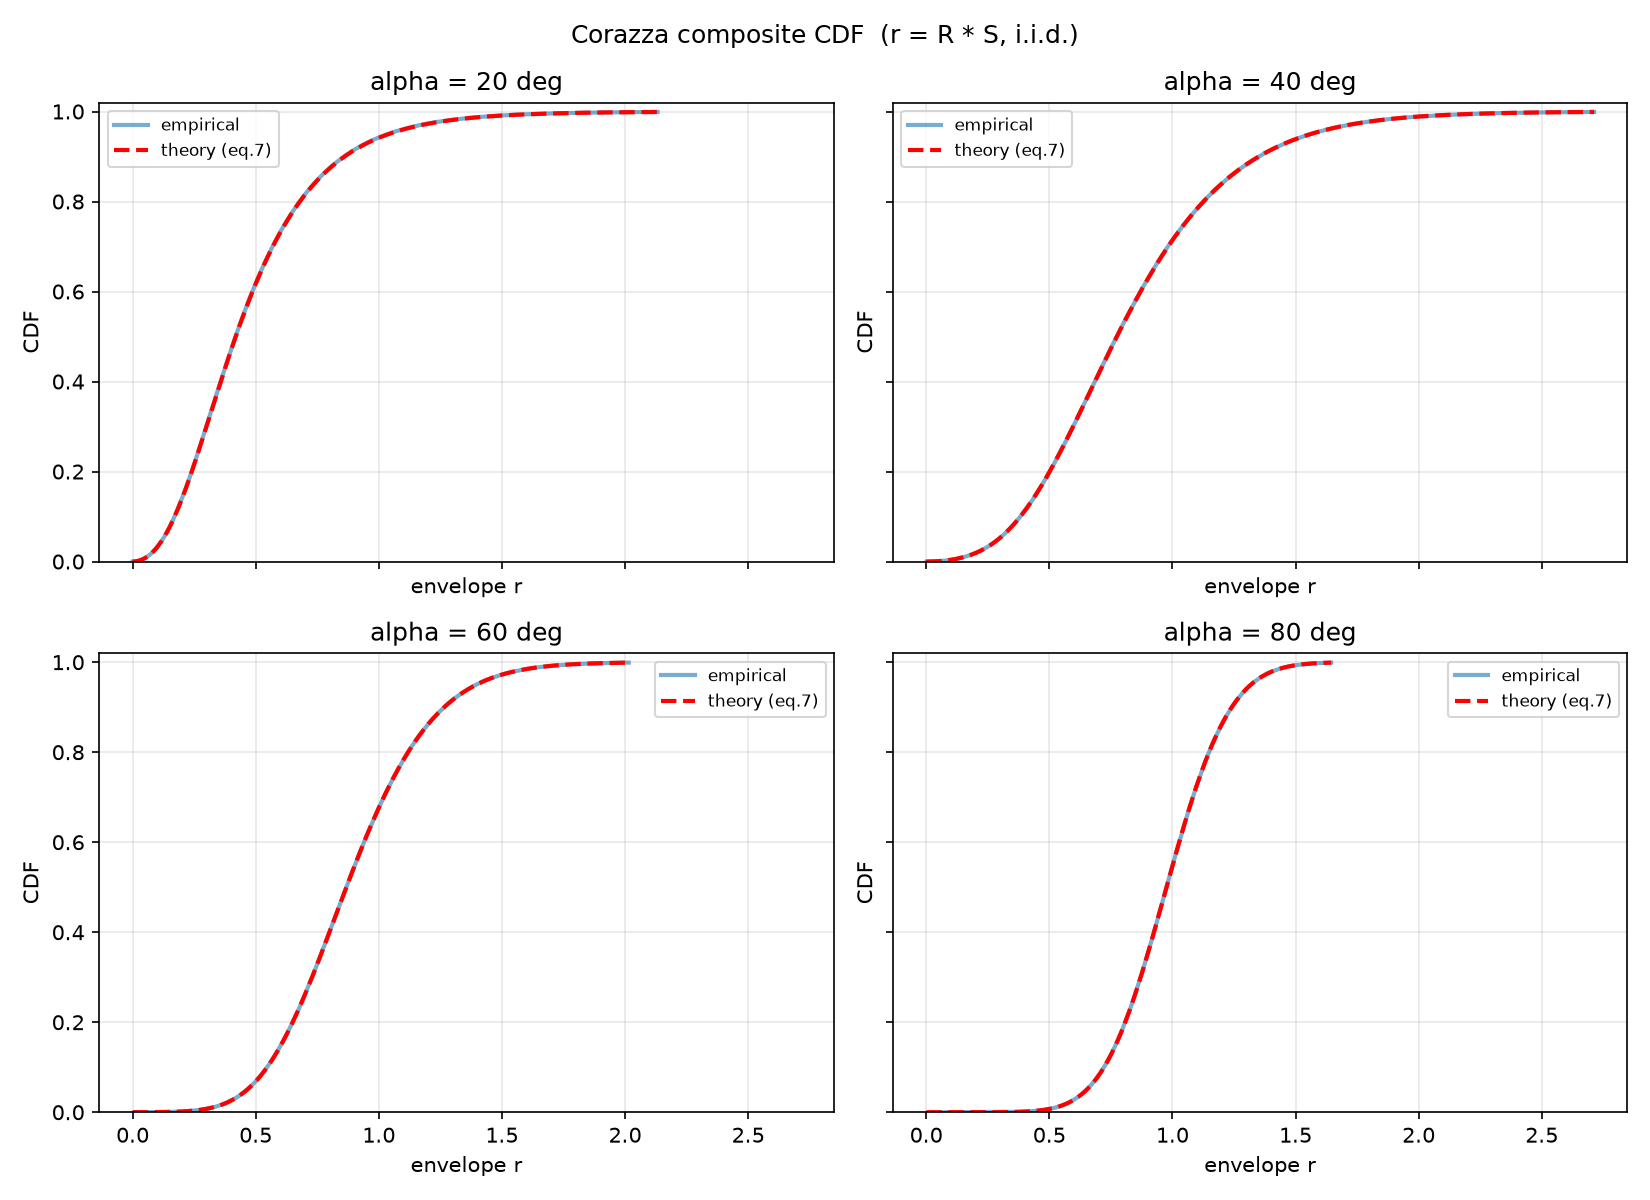
\includegraphics[width=\textwidth]{corazza_cdf.png}\caption{CDF：仿真 vs 理论数值积分}\end{subfigure}
\caption{参考数据质检：不同仰角包络分布与理论对比}
\label{fig:corazza-pdf-cdf}
\end{figure}

\begin{figure}[H]
\centering
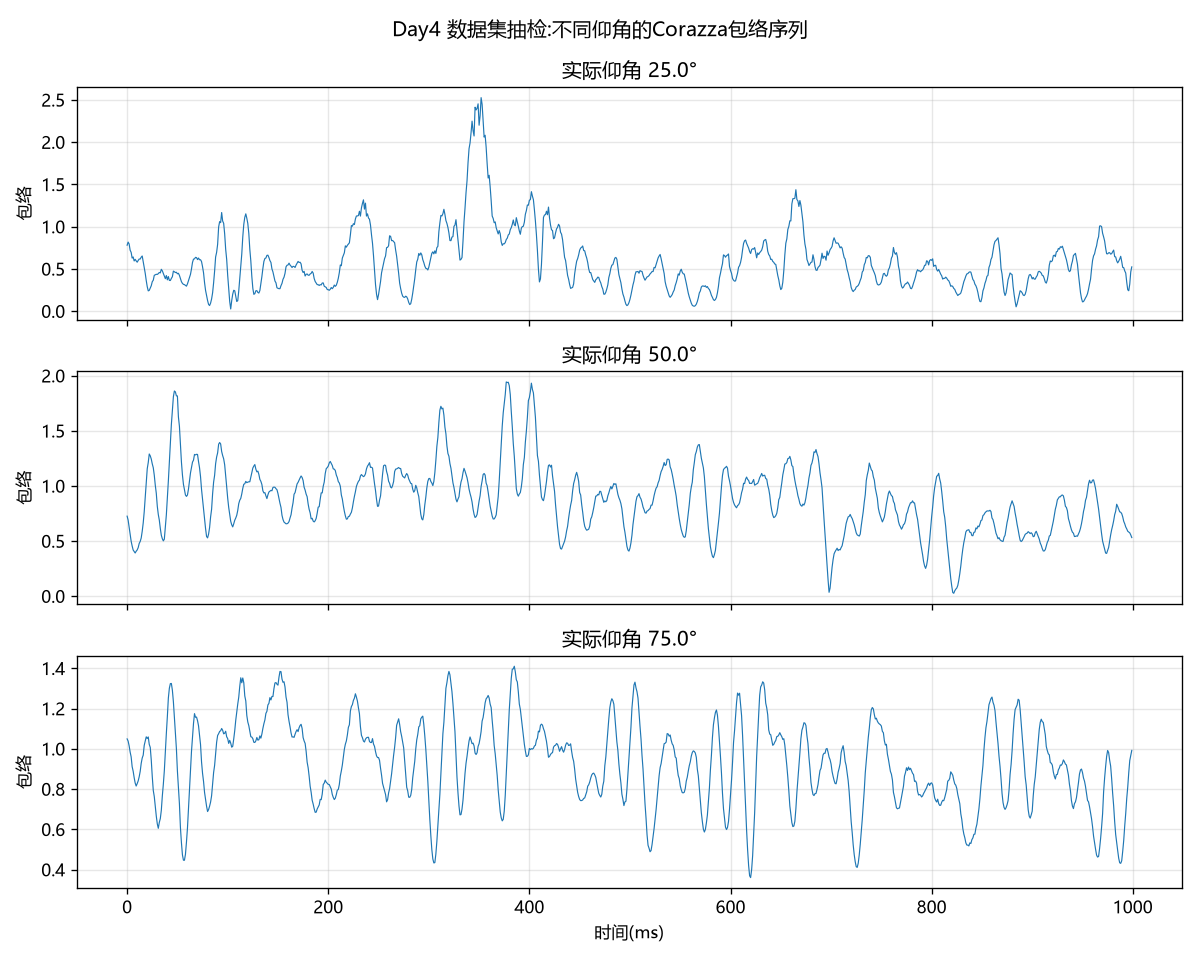
\includegraphics[width=0.8\textwidth]{dataset_samples.png}
\caption{冻结数据集样本示例：不同仰角的包络时序片段}
\label{fig:dataset-samples}
\end{figure}

\subsection{CGAN基线复现结果与条件一致性诊断}
按表\ref{tab:hyper}配置完成CGAN训练（30000步），训练曲线见图\ref{fig:cgan-train}：判别器损失稳定于低位、Wasserstein距离估计收敛到稳定值，训练过程整体可控，未出现模式崩溃。图\ref{fig:cgan-45}a给出代表性仰角45°的生成分布：PDF直方图与参考高度重叠，KS$=0.021$，分布拟合达到文献\cite{chen2026cgan}同量级水平。

\begin{figure}[H]
\centering
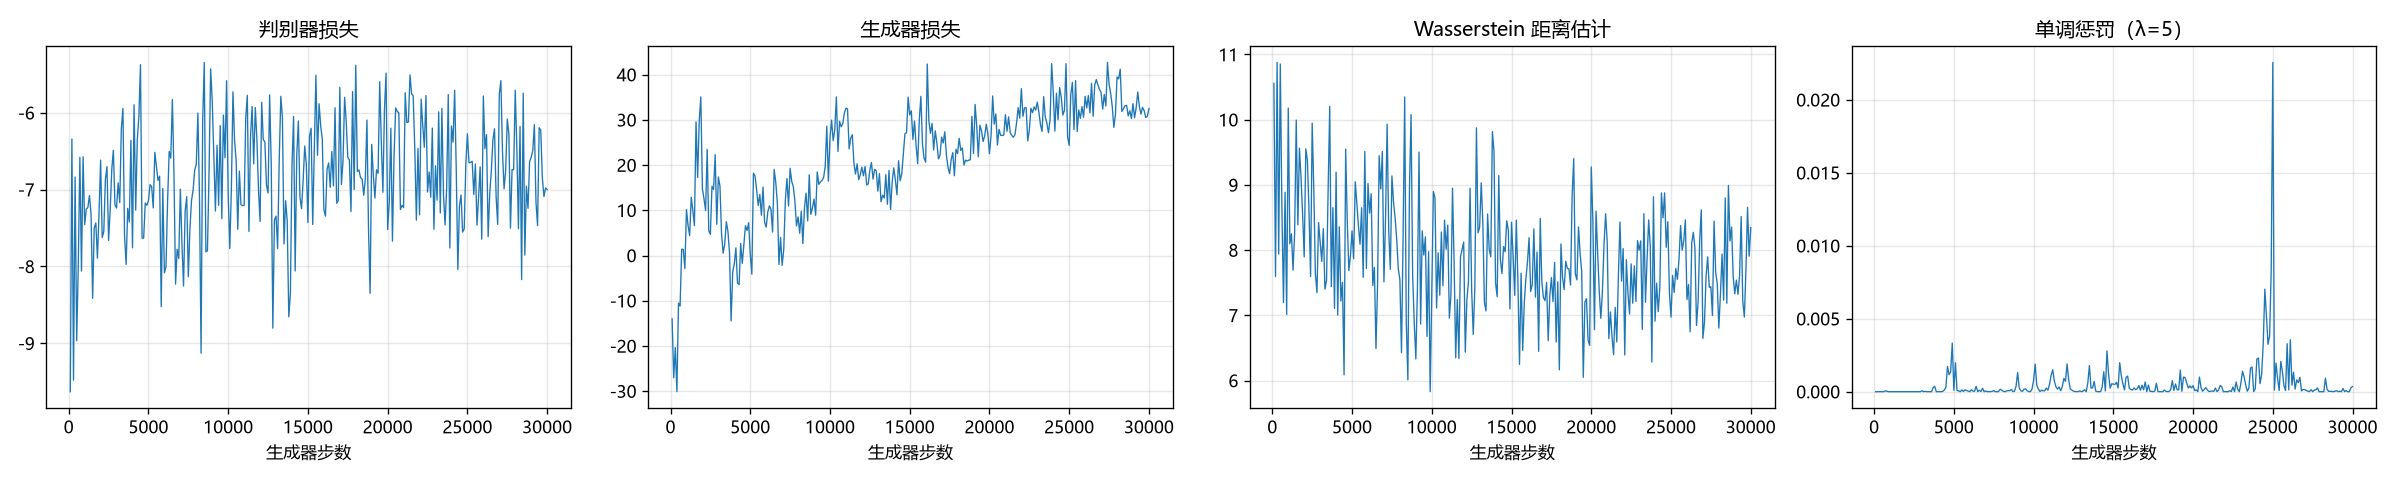
\includegraphics[width=0.62\textwidth]{cgan_train_curves.png}
\caption{CGAN基线复现：训练曲线（判别器/生成器损失与Wasserstein距离估计）}
\label{fig:cgan-train}
\end{figure}

\begin{figure}[H]
\centering
\begin{subfigure}{0.49\textwidth}\centering
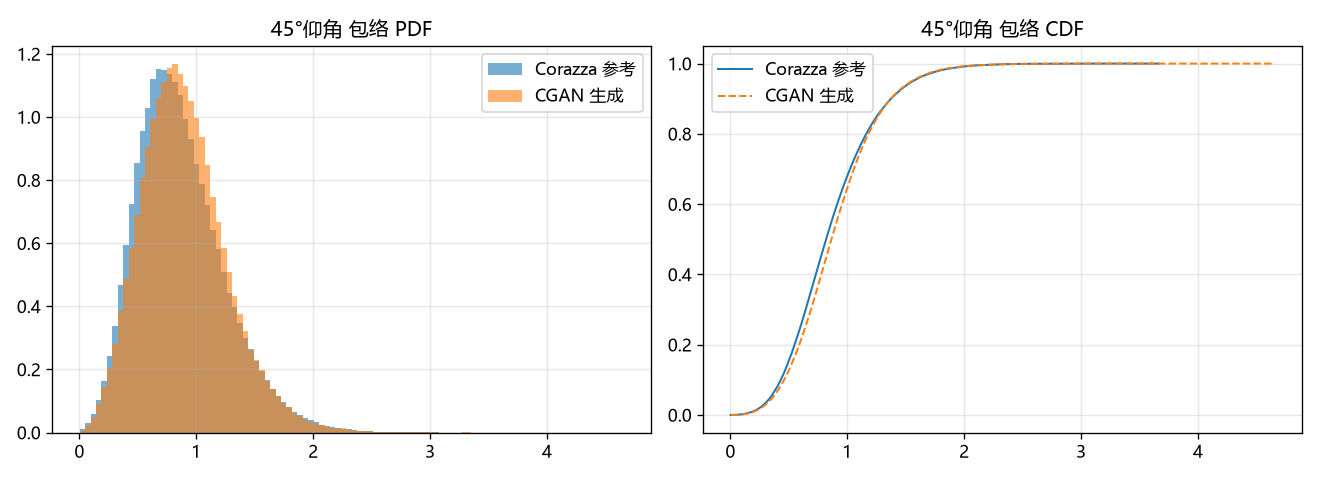
\includegraphics[width=\textwidth]{cgan45_pdfcdf.png}\caption{45°仰角：PDF/CDF对比}\end{subfigure}
\hfill
\begin{subfigure}{0.49\textwidth}\centering
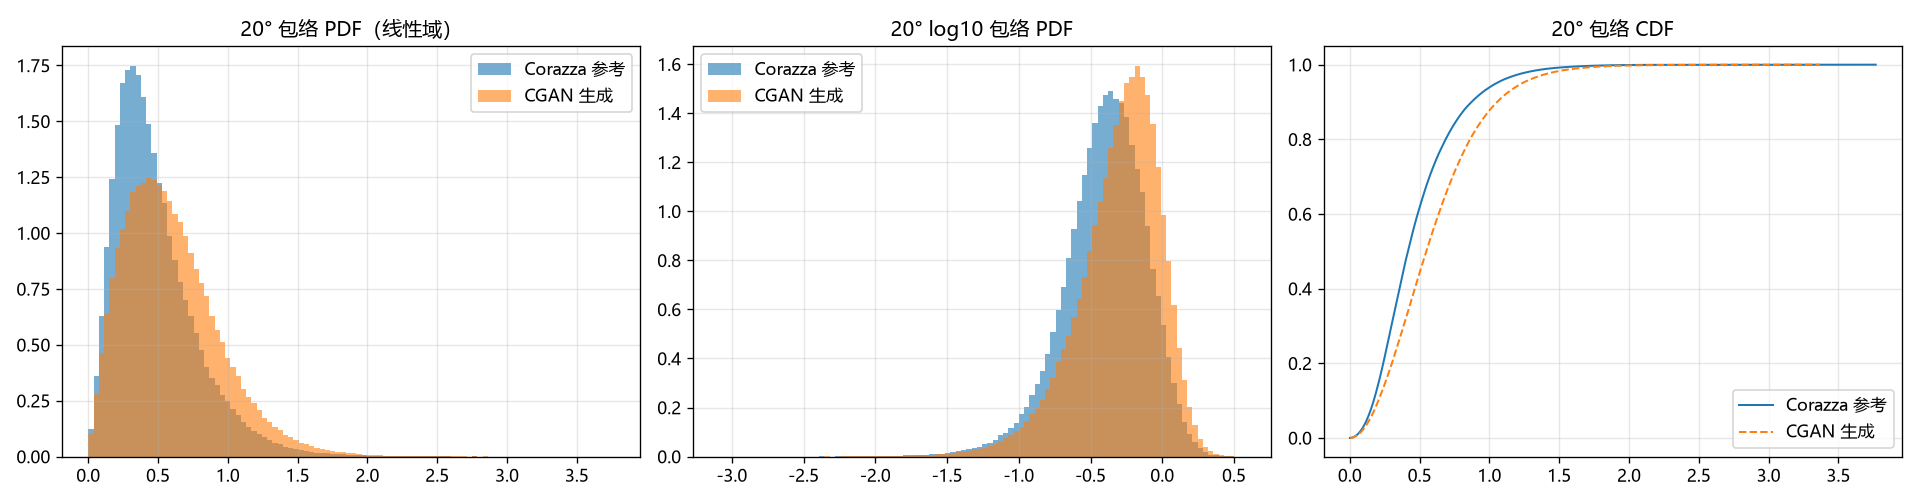
\includegraphics[width=\textwidth]{cgan20_diag.png}\caption{20°仰角分布诊断}\end{subfigure}
\caption{CGAN生成分布检查：(a) 45°仰角PDF/CDF对比；(b) 20°仰角分布诊断}
\label{fig:cgan-45}
\end{figure}

7个测试仰角的逐点验收结果见表\ref{tab:cgan-result}。\textbf{6个仰角KS$<0.07$达到验收线，但30°仰角KS$=0.130$显著超出验收线}；且低仰角整体劣于高仰角。逐仰角诊断（图\ref{fig:cgan-45}b）表明，30°仰角的生成分布相对参考出现系统性偏移。进一步绘制仰角-包络均值曲线（图\ref{fig:mean-curve}）可见：CGAN的均值曲线相对参考出现局部偏离，条件间一致性明显弱于扩散模型。

\begin{table}[H]
\centering\footnotesize
\caption{CGAN基线（文献\,\cite{chen2026cgan}复现）7仰角逐点验收（每仰角500条）}
\label{tab:cgan-result}
\setlength{\tabcolsep}{3pt}
\begin{tabular}{cccccccc}
\toprule
仰角 & KS & PDF $L_1$ & Wasserstein & LCR rel & AFD rel & BER RMSE & 判定\\
\midrule
20° & 0.068 & 0.152 & 0.039 & 0.159 & 0.145 & 0.114 & 通过\\
30° & \textbf{0.130} & 0.260 & 0.109 & 0.328 & 0.270 & 0.153 & \textbf{未通过}\\
40° & 0.044 & 0.099 & 0.027 & 0.271 & 0.597 & 0.112 & 通过\\
50° & 0.018 & 0.046 & 0.014 & 0.236 & 0.167 & 0.039 & 通过\\
60° & 0.024 & 0.095 & 0.017 & 0.173 & — & 0.024 & 通过\\
70° & 0.048 & 0.187 & 0.031 & 0.365 & — & 0.127 & 通过\\
80° & 0.040 & 0.080 & 0.021 & 1.056 & — & 0.022 & 通过\\
\midrule
均值 & 0.053 & 0.132 & 0.038 & 0.370 & — & 0.087 & 6/7\\
\bottomrule
\multicolumn{8}{p{0.98\textwidth}}{\footnotesize 注：AFD在高门限处参考序列无穿越事件，以“—”表示（统计意义缺失，非误差）；验收线见表\ref{tab:accept}。}
\end{tabular}
\end{table}

\textbf{成因分析：}该现象的根源在于WGAN-GP损失的结构性局限——对抗损失仅在\emph{单个}条件下约束分布匹配，缺乏跨条件有序性约束，相邻仰角的生成均值在训练中相互拖拽；条件区间边界（如20°）仅受单侧相邻条件牵制、约束最弱，漂移风险最高。引入跨条件单调一致性正则（同一批噪声跨条件复用，对逆序均值对施加铰链惩罚）可抑制秩翻转，但无法根治单条件内的分布失配（30°仰角KS$=$0.130即加入正则后的结果）。该现象已通过双随机种子（42/1234）复现验证，具有结构性。\textbf{这一发现直接构成本课题引入扩散模型的动机之一}：扩散模型的$\varepsilon$预测回归目标逐条件独立优化，且FiLM条件注入贯穿所有残差块，机理上不存在对抗博弈带来的条件间拖拽。

\begin{figure}[H]
\centering
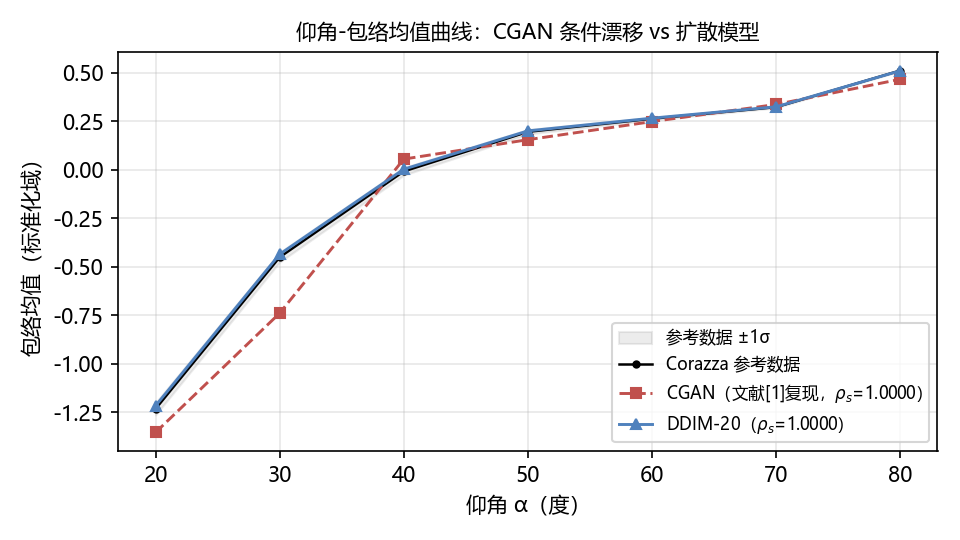
\includegraphics[width=0.78\textwidth]{fig_mean_curve.png}
\caption{仰角-包络均值曲线（标准化域，每仰角500条新采样）：CGAN相对参考出现局部偏离，扩散模型紧贴参考（阴影为参考$\pm1\sigma$）}
\label{fig:mean-curve}
\end{figure}

\subsection{条件扩散模型初步结果}
按表\ref{tab:hyper}完成扩散模型训练。图\ref{fig:ddpm-train}a为训练损失曲线：$\varepsilon$预测MSE平滑单调下降，无对抗训练的震荡，\textbf{训练稳定性显著优于CGAN}。图\ref{fig:ddpm-train}b为DDIM-20步采样在45°的生成分布，KS$=0.014$，已优于CGAN最优仰角。

\begin{figure}[H]
\centering
\begin{subfigure}{0.49\textwidth}\centering
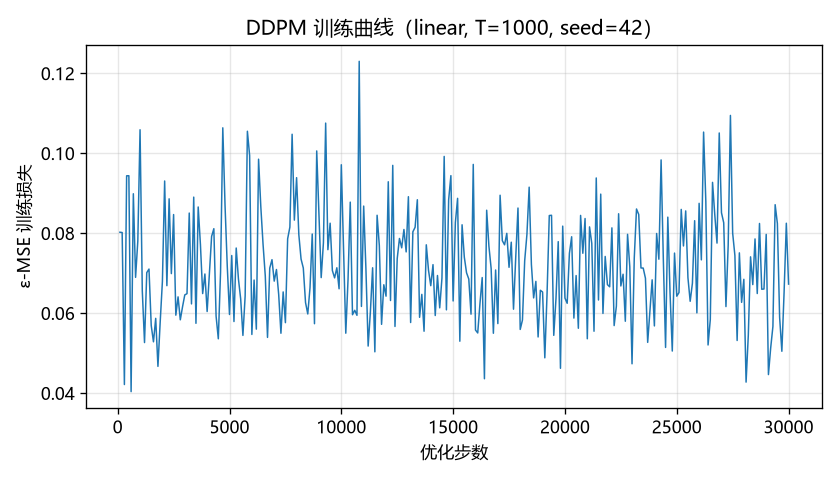
\includegraphics[width=\textwidth]{ddpm_train_curve.png}\caption{扩散模型训练损失（$\varepsilon$-MSE，平滑下降）}\end{subfigure}
\hfill
\begin{subfigure}{0.49\textwidth}\centering
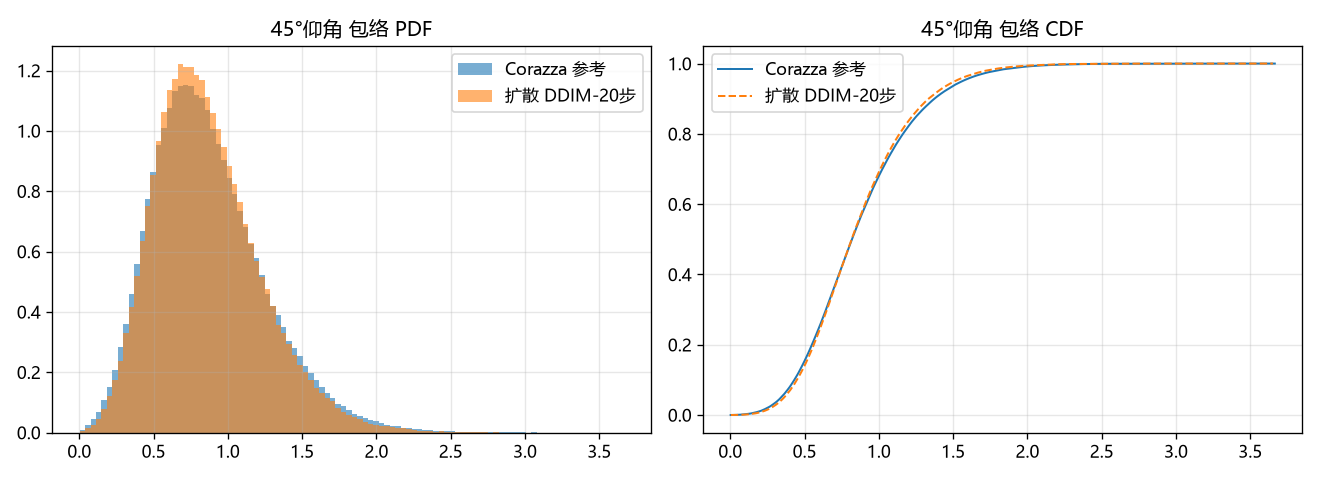
\includegraphics[width=\textwidth]{ddim20_45_pdfcdf.png}\caption{DDIM-20采样45°分布（KS=0.014）}\end{subfigure}
\caption{条件扩散模型：训练过程与代表性采样结果}
\label{fig:ddpm-train}
\end{figure}

图\ref{fig:ks-compare}给出四类配置在7个仰角的KS统计量对比：扩散模型全部配置、全部仰角均通过合格线（0.07），且全部优于优秀线（0.02）；CGAN在30°仰角超出合格线。图\ref{fig:temporal-compare}给出时序指标的对比：扩散模型的LCR相对RMSE在全部仰角低于CGAN，DDPM-1000配置的LCR/AFD相对RMSE均值分别为0.074/0.097，较CGAN（0.370/—）改善一个量级以内但全面占优。各配置汇总见表\ref{tab:diff-result}。

\begin{figure}[H]
\centering
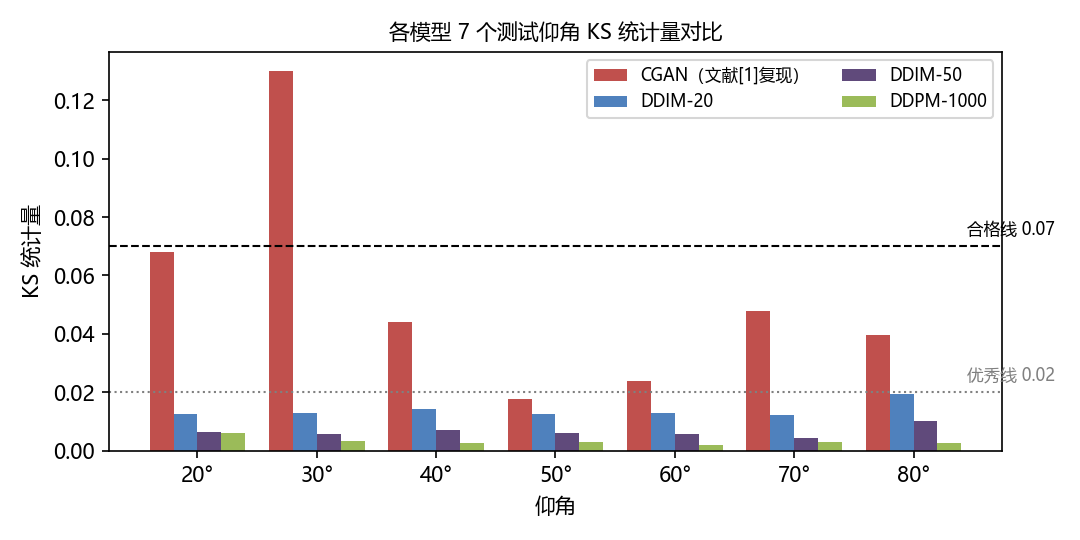
\includegraphics[width=0.86\textwidth]{fig_ks_comparison.png}
\caption{各配置7仰角KS统计量对比：扩散模型全部仰角通过且优于优秀线（0.02），CGAN在30°超出合格线（0.07）}
\label{fig:ks-compare}
\end{figure}

\begin{figure}[H]
\centering
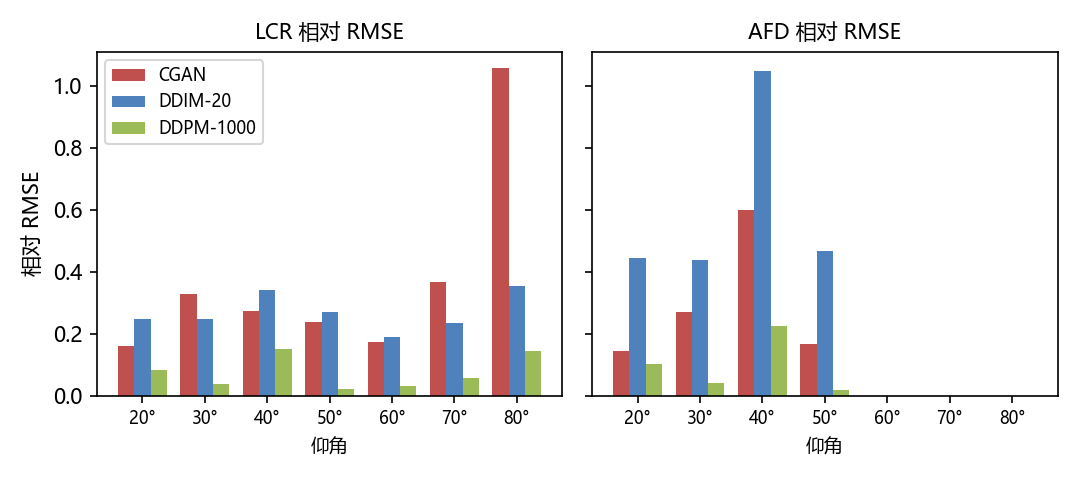
\includegraphics[width=0.86\textwidth]{fig_temporal_comparison.png}
\caption{时序特性指标对比：LCR/AFD相对RMSE（越低越好）}
\label{fig:temporal-compare}
\end{figure}

\begin{table}[H]
\centering\small
\caption{条件扩散模型各采样配置的初步验收汇总（7仰角$\times$500条）}
\label{tab:diff-result}
\begin{tabular}{lccccc}
\toprule
配置 & KS最大 & KS均值 & LCR rel均值 & AFD rel均值 & BER RMSE均值\\
\midrule
DDIM-20 & 0.019 & 0.014 & 0.268 & 0.599 & 0.034\\
DDIM-50 & 0.010 & 0.006 & 0.153 & 0.396 & 0.025\\
DDIM-100 & 0.007 & 0.004 & 0.146 & 0.231 & 0.025\\
DDPM-1000 & 0.006 & 0.003 & 0.074 & 0.097 & 0.020\\
\midrule
CGAN（对照） & \textbf{0.130} & 0.053 & 0.370 & — & 0.087\\
\bottomrule
\multicolumn{6}{l}{\footnotesize 注：AFD均值仅统计有穿越事件的仰角；Spearman $\rho_s$：全部扩散配置$=1.000$，CGAN$\approx0.99$。}
\end{tabular}
\end{table}

\subsection{采样效率基准}
按统一协议（吞吐：每仰角500条、batch=64；延迟：单条45°重复5次取中位数；仅计纯生成时间，cuda同步计时）测定各配置采样成本，结果见表\ref{tab:bench}与图\ref{fig:tradeoff}。

\begin{table}[H]
\centering\small
\caption{采样效率基准（同一GPU环境）}
\label{tab:bench}
\begin{tabular}{lcccc}
\toprule
配置 & 单条延迟(ms) & 批量吞吐(序列/s) & KS均值 & BER RMSE均值\\
\midrule
CGAN & 2.1 & $\approx1.1\times10^{4}$ & 0.053 & 0.087\\
DDIM-20 & 113.5 & 143.8 & 0.014 & 0.034\\
DDIM-50 & 283.9 & 57.3 & 0.006 & 0.025\\
DDIM-100 & 576.4 & 28.7 & 0.004 & 0.025\\
DDPM-1000 & 5722.5 & 2.9 & 0.003 & 0.020\\
\bottomrule
\end{tabular}
\end{table}

\begin{figure}[H]
\centering
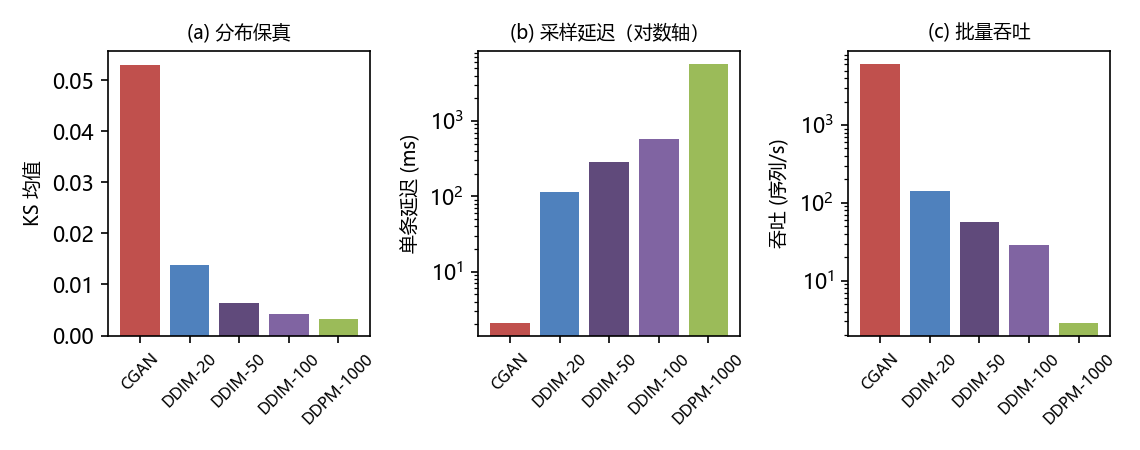
\includegraphics[width=0.95\textwidth]{fig_tradeoff.png}
\caption{质量—成本折中：(a) 分布保真（KS均值）；(b) 单条延迟（对数轴）；(c) 批量吞吐（对数轴）}
\label{fig:tradeoff}
\end{figure}

\textbf{初步分析：}CGAN单条延迟2.1~ms、吞吐逾万条/秒，采样效率优势显著；扩散模型延迟随步数线性增长，DDIM-20（113.5~ms）与CGAN差距约54倍，但批量吞吐（143.8序列/s）已可满足离线批量生成需求。质量维度上，DDIM-20步即满足分布保真（KS均值0.014，优于CGAN的0.053），50步起BER指标反超CGAN均值水平；DDIM-100与DDIM-50的KS几乎持平，表明质量收益在50步后趋于饱和。\textbf{“DDIM-20为离线常规用途的甜点配置”是当前数据支持的初步工程结论}，正式研究将在连续仰角与更大样本量下复核该折中曲线。

\subsection{初步结论与对后续研究的启示}
综合前期结果，可提炼五点初步结论：
\begin{enumerate}
\item \textbf{分布保真}：条件扩散模型全配置、全仰角KS统计量（最大0.019）显著优于CGAN复现结果（均值0.053，30°失败0.130），达到优秀线水平；
\item \textbf{时序保持}：扩散模型LCR/AFD相对RMSE全面低于CGAN，且随采样步数增加持续改善，验证了“迭代去噪机制适配时序相关结构”的研究假设的初步成立方向；
\item \textbf{条件一致性}：扩散模型仰角-均值曲线紧贴参考（$\rho_s=1.000$），CGAN存在条件漂移的结构性短板，两种条件注入机制（通道拼接 vs FiLM）的差异是重要变量；
\item \textbf{训练稳定性}：扩散训练损失平滑单调，CGAN训练需WGAN-GP+TTUR+EMA多重技巧且仍存在条件间拖拽；
\item \textbf{工程成本}：扩散采样延迟约为CGAN的54倍（DDIM-20），质量收益在50步后饱和，存在明确的工程甜点。
\end{enumerate}
上述结论目前基于单数据集（Corazza）、单任务（一维包络）与初步训练配置，正式研究将沿三条线深化：其一，系统性训练调优后复核全部指标并补齐训练稳定性定量对比；其二，开展连续仰角泛化测试与跨数据源稳健性检验；其三，引入实测信道数据检验结论的外部有效性。

%======================= 六 =======================
\section{进度安排与预期目标}

\subsection{前期工作基础}
见第五节：已完成数据管线、指标库、CGAN基线复现与扩散模型初步实现，端到端技术路线已贯通。

\subsection{正式研究进度安排（16周）}
\begin{table}[H]
\centering\small
\caption{正式研究进度安排}
\label{tab:schedule}
\begin{tabular}{c p{0.80\textwidth}}
\toprule
周次 & 工作内容\\
\midrule
第1$\sim$3周 & 条件扩散模型系统性训练与结构消融（在前期初步实现基础上）：噪声schedule、条件注入方式、网络规模\\
第4$\sim$6周 & 扩散模型训练调优与7个测试仰角逐点验收；CGAN对照实验补充（多种子）\\
第7$\sim$8周 & DDIM采样步数—生成质量—采样耗时折中分析（含连续仰角）\\
第9$\sim$10周 & 系统性对比实验与连续仰角泛化测试，归纳两类生成范式的能力边界\\
第11$\sim$13周 & 依托课题组地面站开展真实信道数据采集与预处理（视采集条件），构建实测扩充数据集\\
第14周 & 跨数据源稳健性检验（两模型在新数据集上重训对比）\\
第15$\sim$16周 & 论文撰写、修改定稿与答辩准备\\
\bottomrule
\end{tabular}
\end{table}

\subsection{预期达到的目标}
（1）完成仰角条件扩散模型的系统性训练与调优，7个测试仰角的分布拟合精度达到并保持前期初步结果的优秀线水平（KS$<0.02$）；
（2）在三层指标与工程维度上全面量化对比两类模型的分布拟合精度、时序保持能力、系统性能后果与工程效率，重点检验“扩散模型在时序指标（LCR/AFD相对RMSE）上是否优于CGAN基线”这一研究假设；
（3）完成真实信道数据采集（视采集条件）与跨数据源稳健性检验，形成完整的三层评价对比实验报告（含采样步数—生成质量—采样耗时折中曲线）与可复现代码库；
（4）完成毕业论文一篇。

%======================= 七 =======================
\section{课题已具备和所需的条件、经费}

\textbf{已具备的条件：}
（1）方法与数据基础：文献\cite{chen2026cgan}已公开全部数据规格、训练超参与评价指标定义，本课题已完成其方法体系梳理与CGAN基线复现，数据管线与三层评价指标库经回归测试后冻结，复现要件完整、对比基准可信；
（2）前期验收基础：复现的CGAN基线在7个测试仰角中6个达到文献\cite{chen2026cgan}同量级水平，条件扩散模型初步实现已在全部仰角通过优秀线验收，验证了数据管线、指标库与训练流程的端到端可行性，为16周进度安排的任务分解与工作量估计提供了可靠基础；
（3）算力与工具条件：实验所用GPU算力已具备，PyTorch等开源深度学习工具链成熟，可满足生成模型训练与大规模采样评估的算力需求。

\textbf{所需条件与经费：}本课题全程基于开源软件工具链与课题组既有资源，无元器件、设备采购需求，无需经费支持；真实信道数据采集拟依托课题组地面站资源实施（视采集条件安排），均不涉及经费。

%======================= 八 =======================
\section{研究过程中可能遇到的困难和问题，解决的措施}

\textbf{（1）WGAN-GP的条件间一致性难以保证。}对抗损失仅在单个条件下约束分布匹配，缺乏跨条件有序性约束，前期复现过程中已观察到相邻仰角条件均值互相拖拽、条件均值曲线局部偏离的现象，30°仰角KS$=0.130$超出验收线。解决措施：沿用文献\cite{chen2026cgan}已验证的WGAN-GP、TTUR与EMA组合并以EMA权重采样抑制波动，辅以训练全程的条件均值曲线与逐仰角KS/Spearman监测；引入跨条件单调一致性正则约束相邻仰角的均值顺序；该现象同时作为GAN类方法的结构性局限纳入对比分析（已部分完成）。

\textbf{（2）扩散模型训练与采样计算开销大。}DDPM反向采样需千步迭代，生成效率远低于CGAN单次前向（前期实测单条延迟差距约54倍）。解决措施：采用DDIM确定性采样将步数压缩至数十步量级，控制U-Net规模与训练序列长度，并系统测定“采样步数—生成质量—采样耗时”折中曲线（前期已获初步折中数据，正式研究将扩展至连续仰角），为生成模型的工程选型提供依据。

\textbf{（3）时序指标的统计精度与计算成本相互制约。}LCR/AFD属稀有事件计数统计，相对统计误差随样本量按$1/\sqrt{N}$标度，往往需要大样本（十万级）才能可靠区分模型差异；而逐样本点的数值积分在大样本量下计算量巨大。解决措施：评估前按样本量校准指标阈值，采用网格插值将数值积分次数由样本量级降至网格量级，兼顾统计精度与计算开销，并以冻结数据集保证回归测试可复现（前期已验证该方案）。

\textbf{（4）缺乏同频段同场景的公开实测数据。}Corazza模型参数依赖特定测量场景拟合，参考数据与真实信道的偏差会传导至生成模型的评估结论。解决措施：视采集条件，依托课题组地面站资源自采实测数据作为补充验证；论文中对数据局限如实说明。

\textbf{（5）公平对比的口径控制。}两模型对比结论的有效性完全取决于数据、指标、种子口径的一致性。解决措施：统一冻结训练集与评价代码，指标接口冻结后任何变更必须重跑全量回归测试并登记变更日志。

%======================= 九 =======================
\section{主要参考文献}
\begin{thebibliography}{99}
\sloppy
\setlength{\itemsep}{-0.3ex}
\small
\bibitem{chen2026cgan} 陈万埼. 基于CGAN的NGSO星座星地信道建模方法与仿真[D]. 哈尔滨: 哈尔滨工业大学, 2026.
\bibitem{loo1985statistical} Loo C. A statistical model for a land mobile satellite link[J]. IEEE Transactions on Vehicular Technology, 1985, 34(3): 122-127.
\bibitem{lutz1991land} Lutz E, Cygan D, Dippold M, et al. The land mobile satellite communication channel: recording, statistics, and channel model[J]. IEEE Transactions on Vehicular Technology, 1991, 40(2): 375-386.
\bibitem{corazza1994statistical} Corazza G E, Vatalaro F. A statistical model for land mobile satellite channels and its application to nongeostationary orbit systems[J]. IEEE Transactions on Vehicular Technology, 1994, 43(3): 738-742.
\bibitem{fontan2001statistical} Fontán F P, Vázquez-Castro M, Cabado C E, et al. Statistical modeling of the LMS channel[J]. IEEE Transactions on Vehicular Technology, 2001, 50(6): 1549-1567.
\bibitem{abdi2003new} Abdi A, Lau W C, Alouini M S, et al. A new simple model for land mobile satellite channels: first- and second-order statistics[J]. IEEE Transactions on Wireless Communications, 2003, 2(3): 519-528.
\bibitem{3gpp38811} 3GPP. Study on New Radio (NR) to support non-terrestrial networks: TR 38.811[R]. 2020.
\bibitem{itu618} ITU-R. Propagation data and prediction methods required for the design of Earth-space telecommunication systems: Recommendation P.618[S]. 2023.
\bibitem{baeza2022overview} Baeza V M, Lagunas E, Al-Hraishawi H, et al. An overview of channel models for NGSO satellites[C]//2022 IEEE 96th Vehicular Technology Conference (VTC2022-Fall). IEEE, 2022: 1-6.
\bibitem{goodfellow2014generative} Goodfellow I, Pouget-Abadie J, Mirza M, et al. Generative adversarial nets[C]//Advances in Neural Information Processing Systems, 2014, 27: 2672-2680.
\bibitem{xiao2022channelgan} Xiao H, Tian W, Liu W, et al. ChannelGAN: Deep learning-based channel modeling and generating[J]. IEEE Wireless Communications Letters, 2022, 11(3): 650-654.
\bibitem{cheng2022gan} 程芳芳. 基于GAN网络的无线信道建模方法研究[D]. 大连: 大连海事大学, 2022.
\bibitem{qiao2023leo} 乔艳丽. 低轨卫星移动信道建模与仿真实现[D]. 北京: 北京邮电大学, 2023.
\bibitem{gulrajani2017improved} Gulrajani I, Ahmed F, Arjovsky M, et al. Improved training of Wasserstein GANs[C]//Advances in Neural Information Processing Systems, 2017, 30: 5767-5777.
\bibitem{ho2020denoising} Ho J, Jain A, Abbeel P. Denoising diffusion probabilistic models[C]//Advances in Neural Information Processing Systems, 2020, 33: 6840-6851.
\bibitem{song2021denoising} Song J, Meng C, Ermon S. Denoising diffusion implicit models[C]//International Conference on Learning Representations, 2021.
\bibitem{dhariwal2021diffusion} Dhariwal P, Nichol A. Diffusion models beat GANs on image synthesis[C]//Advances in Neural Information Processing Systems, 2021, 34: 8780-8794.
\bibitem{tian2026scalable} Tian J, Cai L. Scalable air-to-ground wireless channel modeling using environmental context and generative diffusion[EB/OL]. arXiv:2603.24620, 2026[2026-10-12]. https://arxiv.org/abs/2603.24620.
\bibitem{huang2026physics} Huang X, Zhang Y, Qin X, et al. Physics-informed digital twins for channel estimation and traffic prediction of non-terrestrial networks[EB/OL]. arXiv:2605.23155, 2026[2026-10-12]. https://arxiv.org/abs/2605.23155.
\bibitem{xia2025leo} Xia T, et al. LEO satellite channel modeling based on latent diffusion models and PINNs[C]//IEEE SPCT. IEEE, 2025.
\end{thebibliography}

\end{document}
